\subsection{Amdahl's and Gustafson's Laws}

The \definition{Amdahl's Law} is a formula which gives the \textbf{theoretical speedup in latency of the execution of a task at fixed workload that can be expected of a system whose resources are improved}. The law can be stated as:
\begin{definitionbox}[: Amdahl's Law]
    \textbf{The overall performance improvement gained by optimizing a single part of a system is limited by the fraction of time that the improved part is actually used.}
\end{definitionbox}

\noindent
In practice, Amdahl's law says that the computation consists of interleaved segments of two types:
\begin{enumerate}
    \item \textbf{Serial segments} (which cannot be parallelized);
    \item \textbf{Parallelizable segments}.
\end{enumerate}
Therefore, the metrics we can obtain are the time on $P$ processors metric, that it is greater than the fraction of time on a processor divided by the processors $P$, and the speedup metric, that it is less than the number of processors $P$:
\begin{equation*}
    T_{P} > \dfrac{T_{1}}{P} \hspace{2em} SU < P
\end{equation*}
Graphically, we can see a fixed part of the line, which is the \textbf{serial segment} (no speedup), and a set of instructions that can be \textbf{parallelized} (the sum of these segments is equal to the unit time $1$).
\begin{figure}[!htp]
    \centering
    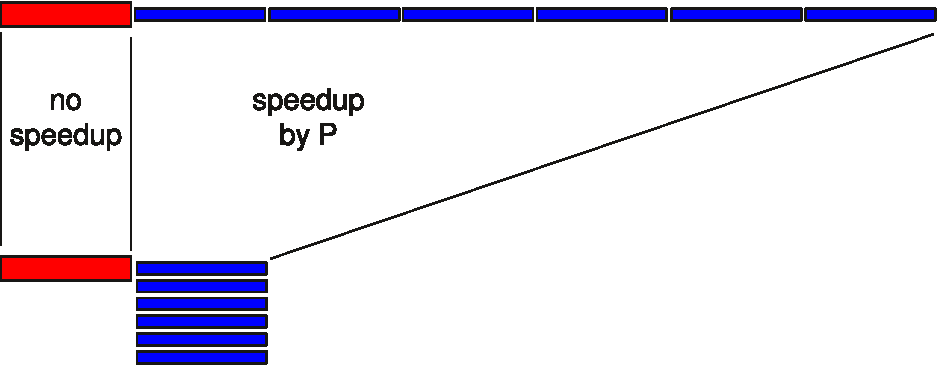
\includegraphics[width=\textwidth]{img/amdahl-law-1.pdf}
\end{figure}

\noindent
Furthermore, if we identify the parallelizable segment as $f$ and the serial segment as $1-f$, we obtain the following expressions:
\begin{equation}
    \begin{array}{rcl}
        SU\left(P,f\right) &=& \dfrac{T_{1}}{T_{P}} = \dfrac{T_{1}}{T_{1} \cdot \left(1-f\right) + \frac{T_{1}\cdot f}{P}} = \dfrac{1}{\left(1-f\right) + \frac{f}{P}} \\ [1em]
        \lim\limits_{P \rightarrow \infty}SU\left(P,f\right) &=& \dfrac{1}{1-f}
    \end{array}
\end{equation}

\highspace
In the following figure we can see the speedup with parameter $f$. Note the pessimism: for a problem with inherent $f=90\%$, there is no point in using more than 10 processors.
\begin{figure}[!htp]
    \centering
    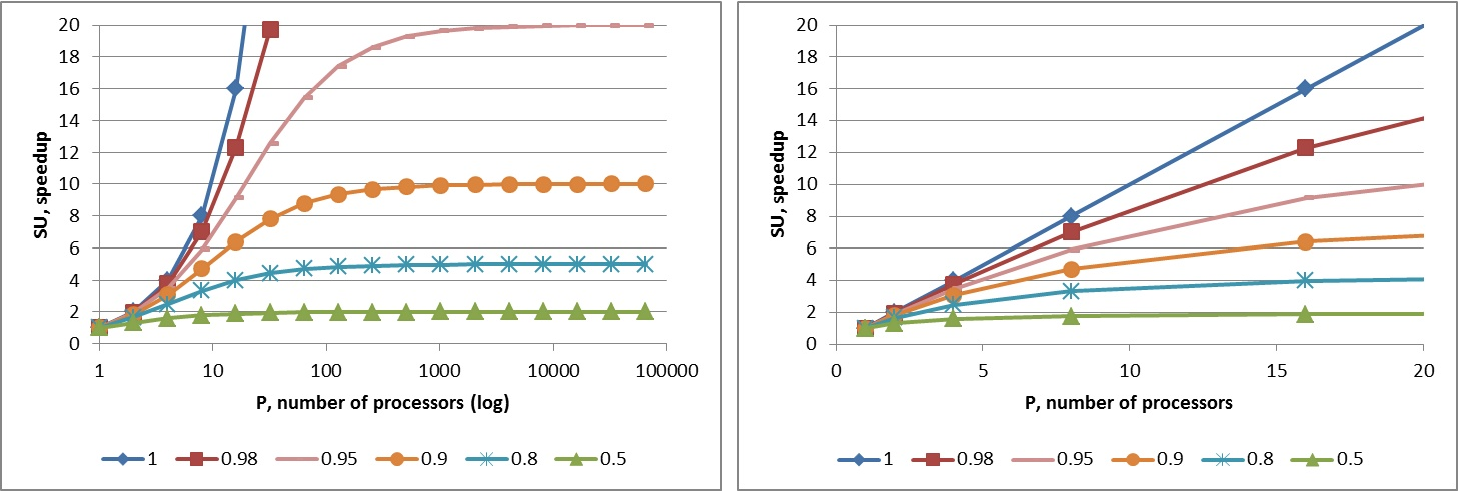
\includegraphics[width=\textwidth]{img/amdahl-law-2.pdf}
    \caption{Amdahl's law, $SU\left(P\right)$, parameter $f$.}
\end{figure}

\noindent
The original paper presenting Amdahl's Law\cite{amdahl2007validity} can be viewed by clicking on the link below or by scanning the QR code.
\begin{center}
    \href{https://ieeexplore.ieee.org/abstract/document/4785615}{Amdahl's Law}
    \hspace{2em}
    \qrcode{https://ieeexplore.ieee.org/abstract/document/4785615}
\end{center}
\textbf{Amdahl's law applies only to the cases where the problem size is fixed}. In practice, as more computing resources become available, they tend to get used on larger problems (larger datasets), and the time spent in the parallelizable part often grows much faster than the inherently serial work. In this case, \textbf{Gustafson's law gives a less pessimistic and more realistic assessment of the parallel performance}.\cite{mccool2012structured}

\highspace
\definition{Gustafson's Law} gives the speedup in the execution time of a task that theoretically gains from parallel computing, using a hypothetical run of the task on a single-core machine as the baseline. To put it another way, it is the \textbf{theoretical \dquotes{slowdown} of an already parallelized task if running on a serial machine}.

\highspace
Against Amdahl's law, Gustafson suggests the following ideas:
\begin{itemize}
    \item Portion $f$ is not fixed;
    \item The absolute serial time is fixed;
    \item Parallel problem size is increased to exploit more processors;
    \item Fixed serial time ($s$ of total) and fixed parallel time ($1-s$ of total) are invariants;
    \item \textbf{Fixed time model} and not fixed size model (as Amdahl's law):
    \begin{equation}
        SU\left(P\right) = \dfrac{T_{1}}{T_{P}} = \dfrac{s+P\cdot\left(1-s\right)}{s+\left(1-s\right)} = s + P\cdot\left(1-s\right)
    \end{equation}
\end{itemize}

\newpage

\noindent
Gustafson's law suggests a \textbf{linear speedup} and is \textbf{empirically applicable to highly parallel algorithms}.
\begin{figure}[!htp]
    \centering
    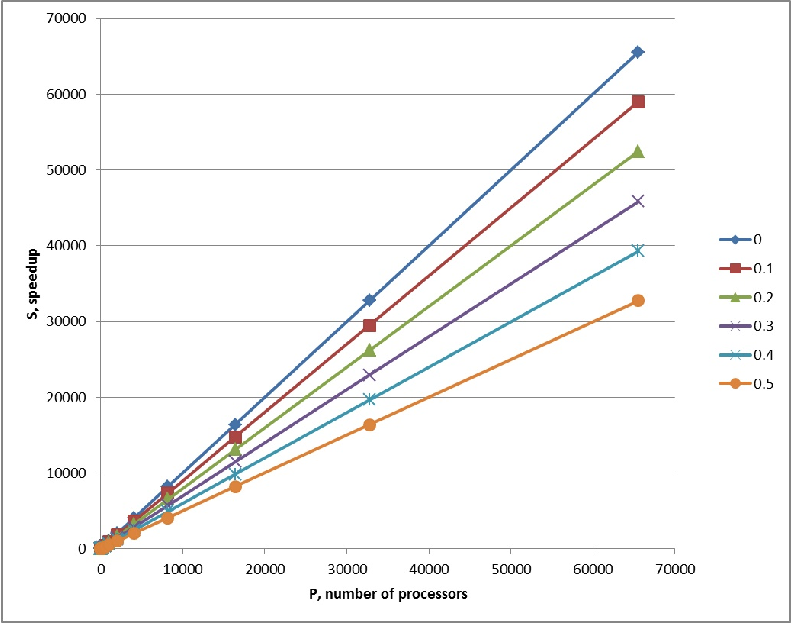
\includegraphics[width=.7\textwidth]{img/gustafson-law-1.pdf}
    \caption{Gustafson's law.}
\end{figure}

\noindent
\textbf{\emph{Amdahl's Law}} states that as computing power increases, computational requirements remain the same. In other words, the \textbf{analysis of the same data will take less time with more computing power}.

\textbf{\emph{Gustafson}}, on the other hand, argues that \textbf{more computing power leads to more careful and complete analysis of the data}. Where it would not have been possible or practical to simulate the impact of nuclear denotation on every building, car, and their contents (including furniture, structural strength, etc.) because such a calculation would have taken more time than was available to provide an answer, the increase in computing power will prompt researchers to add more data to more fully simulate more variables, giving a more accurate result.

\highspace
The original paper presenting Gustafson's Law\cite{gustafson1988reevaluating} can be viewed by clicking on the link below or by scanning the QR code.
\begin{center}
    \href{https://dl.acm.org/doi/abs/10.1145/42411.42415}{Gustafson's Law}
    \hspace{2em}
    \qrcode{https://dl.acm.org/doi/abs/10.1145/42411.42415}
\end{center}